\section{摘要}\label{ux6458ux8981}

语音科学实验常常需要合成刺激：它们既要足够自然，以便被试能够反复听辨，又要能够沿着语音学上有意义的维度进行显式控制，例如基频、共振峰频率、谱倾斜、强度和嗓音质量。现代神经声码器能够提供较高的感知质量，但其数据需求和潜在声学表征往往使其难以直接用于小数据语音学研究。经典共振峰合成具有可解释性和可控性，但通常缺乏生态有效实验刺激所需的自然度。本文提出
ARIA-NSF：一种面向小数据、单说话人语音学刺激生成的可微 Klatt
风格神经源-滤波合成器。

ARIA-NSF 的核心是双混合结构：声源侧使用由 \(F_0\) 和 \(R_d\) 控制的解析
LF 声门激励、整形噪声，以及带状非周期性（band aperiodicity,
AP）混合权重；滤波侧使用确定性共振峰/全极点段与学习残差 biquad
共同构成声道级联。在当前 F024 16 kHz 主配置 v4
中，声道级联包含三个确定性 biquad
段（谱倾斜、\(F_1\)、\(F_2\)）和六个学习 biquad 段，对应名义 LPC 阶数
\(2(3+6)=18\)。22/24 kHz 的 v1/v3/v4/v5 配置使用八个学习
biquad，对应名义 22 阶；v2 因关闭谱倾斜而使用九个学习 biquad，同样保持
22 阶。先导评测显示，F024 v4 在描述性复制合成评测中的 MCD/MSS-STFT
数值较低，F1/F2 操控达到 \(R^2=0.890/0.986\)，模型规模约 5.6M
可训练参数。本文将这些结果作为系统性先导证据，而不是最终感知结论：当前仍缺少人类听测，部分自然度结果来自
UTMOS 等神经代理指标，且若干评估尚非 held-out 泛化结果。

\textbf{关键词：} 神经源-滤波模型；共振峰合成；可微
DSP；语音学刺激生成；小数据语音合成；嗓音质量

\section{1. 引言}\label{ux5f15ux8a00}

可控语音合成处在语音技术与语音科学之间一个特殊的位置。在文本转语音和神经声码器中，主要目标通常是感知自然度、说话人相似性或大规模泛化能力。然而，在语音学和心理语言学实验中，研究目标往往不同：刺激需要足够自然，能够被反复听辨，但实验操控本身也必须可解释、精确，并且最好是低维的。语音学家可能需要调节
\(F_0\) 轨迹来构造声调或语调连续统，独立改变 \(F_1\) 和 \(F_2\)
来构造元音连续统，或调节声源相关参数以研究气声、嘎裂声和紧嗓音等发声类型（breathy,
creaky, pressed
voice）。因此，一个能够生成合理音频、但把这些变量隐藏在高维潜在表征中的系统，并不总是适合实验工作。

这种需求在典型的语音科学场景中尤其具有挑战性。与现代语音生成流程不同，实验材料往往是为了某个具体研究而采集的，而不是来自数十小时或数千小时的大规模训练数据。一个数据集可能只包含来自单一说话人的
5--60
分钟语音，且录制设计围绕一个特定现象，例如连读变调、范畴感知、韵律重音、元音归一化或发声类型。这类数据的价值正在于它们服务于一个清晰假设，但它们通常太小，难以支撑大型通用神经声码器而不出现过拟合、伪影或可控性损失。

经典源-滤波理论 (\citeproc{ref-fant1960acoustic}{Fant 1960})
和共振峰合成 (\citeproc{ref-klatt1980software}{Klatt 1980})
为此提供了基本概念单元：声源、声道滤波器和可解释的声学控制。Praat
(\citeproc{ref-boersma2001praat}{Boersma 2001})
等工具仍然是语音学中的核心工具，因为它们支持语音学家能够理解的分析和操控方式。然而，纯经典合成听感往往不够自然，尤其是在用于生成完整实验刺激而非孤立演示时。相反，现代神经声码器和神经源-滤波模型能够生成高质量波形
(\citeproc{ref-wang2020nsf}{Wang et al.
2020})，但它们的控制变量通常没有与实验操控直接对应。

本文提出 ARIA-NSF，一种小数据可微 Klatt
风格神经源-滤波合成器。其核心设计思想是：语音学刺激生成需要清晰的模块分工，即将具有明确声学机制的实验变量保持为解析或确定性控制，而将音色和频谱细节中的残差部分交由数据驱动模型学习。在当前实现中，\(F_0\)、\(F_1\)、\(F_2\)、带宽、增益、谱倾斜和声门源参数都作为可控变量显式提供；一个小型神经模型预测或细化复制合成所需的其余控制量。

ARIA-NSF
更适合被描述为结构上的双混合模型，而不是确定性成分与神经成分之间字面意义上的
50/50 切分。在声源侧，周期性声门源由 \(F_0\) 和 \(R_d\)
确定性生成，噪声谱形和 AP
混合由模型学习或条件化得到。在滤波侧，对实验重要的声道控制保持确定性和可解释性，而学习残差
biquad
用于提供说话人特异的频谱细节。因此，该模型在声源侧和滤波侧均采用了解析成分与学习成分的分工：显式
DSP
模块保留需要人工编辑的实验变量，神经残差模块建模难以手工指定的频谱细节。

本文的目标并不是构建一个通用 TTS 系统。相反，ARIA-NSF
面向一个更窄但常见的研究用例：从小规模单说话人语料中创建可解释、可操控、客观重建质量较稳的语音刺激。本文最强的主张是架构性主张；经验结果应被理解为先导证据，而不是封闭基准测试。本文的贡献包括：

\begin{enumerate}
\def\labelenumi{\arabic{enumi}.}
\tightlist
\item
  将语音学刺激生成定义为不同于通用 TTS
  的约束问题：小数据、显式干预、低耦合、残差自然度和实验室可训练性。
\item
  提出一种可微 Klatt
  风格双混合架构，在声源侧和滤波侧均采用``解析可控变量 +
  学习残差容量''的模块分工。
\item
  汇总普通话 F024
  数据集及跨语料先导证据链，覆盖复制合成质量、参数操控可靠性、不期望声学耦合、代理自然度指标和主要限制。
\end{enumerate}

\section{2. 相关工作}\label{ux76f8ux5173ux5de5ux4f5c}

\subsection{2.1
经典共振峰合成与语音学操控}\label{ux7ecfux5178ux5171ux632fux5cf0ux5408ux6210ux4e0eux8bedux97f3ux5b66ux64cdux63a7}

语音产生的源-滤波模型将语音描述为喉部声源与声道滤波器之间的相互作用
(\citeproc{ref-fant1960acoustic}{Fant 1960})。Klatt
的级联/并联共振峰合成器 (\citeproc{ref-klatt1980software}{Klatt 1980})
将这一理论操作化，暴露出共振峰频率、带宽、浊音幅度、送气、擦音和谱倾斜等参数。对语音学实验而言，这种控制层级很有吸引力，因为研究者可以操控一个声学维度，同时近似保持其他维度不变。

其限制在于感知质量。即使一个经典共振峰合成器准确实现了某个声学假设，生成的刺激也可能以影响听者行为的方式显得合成化。这一点很重要，因为感知实验不仅测试声学可辨性，也嵌入在听者对自然语音的预期之中。带有明显伪影的刺激连续统可能会混淆原本想要检验的操控。

Praat (\citeproc{ref-boersma2001praat}{Boersma 2001}) 和基于 LPC
的复制合成之所以仍然广泛使用，是因为它们可以实际地分析和操控音高及共振峰相关属性。然而，逆滤波和源-滤波分离并不完美。如果残差信号中仍然保留共振峰信息，共振峰操控就可能引入伪影或意外的声学耦合。

\subsection{2.2 神经源-滤波与可微 DSP
模型}\label{ux795eux7ecfux6e90-ux6ee4ux6ce2ux4e0eux53efux5fae-dsp-ux6a21ux578b}

神经源-滤波模型将语音产生结构重新引入神经波形生成。Wang 等人
(\citeproc{ref-wang2020nsf}{2020}) 提出了 NSF
框架，其中源模块生成激励信号，神经滤波模块将其转换为波形，条件模块对声学特征进行预处理。该设计保留了由
\(F_0\) 驱动的显式激励，同时避免了自回归生成。

可微数字信号处理（DDSP）同样主张，将已知信号处理算子嵌入可训练系统能够帮助神经音频模型
(\citeproc{ref-engel2020ddsp}{Engel et al. 2020})。DDSP
系统并不把整个波形生成器作为无约束网络来学习，而是学习可解释模块的控制参数，例如振荡器、滤波器和混响。这一点对于小数据场景尤其相关，因为归纳偏置能够减少训练可用合成器所需的数据量。

GOLF (\citeproc{ref-yu2024golf}{Yu and Fazekas 2024})
是一个非常接近的参考点。它使用声门流波表作为谐波源，并使用 LPC
滤波器来建模声道，从而实现紧凑高效的歌声合成器。GOLF
表明，语音产生约束可以整合进可微合成，同时保持有竞争力的质量和效率。ARIA-NSF
遵循相同的一般思想，但目标是语音科学刺激生成而非歌声合成，并优先考虑对
\(F_0\)、\(F_1/F_2\) 和声源形状参数的显式操控。

HiFi-Glot (\citeproc{ref-gu2026hifiglot}{Gu et al. 2026})
从高保真神经共振峰合成方向处理了相关问题。它将神经激励与可微共振/全极点滤波器结合，在高感知质量下提供显式共振峰控制。与这类全频带、大容量系统相比，ARIA-NSF
有意保持更小、更专门化。它牺牲一定通用性，以换取小数据可训练性、显式实验控制，以及更接近传统共振峰合成的结构。

\subsection{2.3
混合源-滤波模型中的定位}\label{ux6df7ux5408ux6e90-ux6ee4ux6ce2ux6a21ux578bux4e2dux7684ux5b9aux4f4d}

uSFGAN 中使用的源-滤波分类法 (\citeproc{ref-yoneyama2021usfgan}{Yoneyama
et al. 2021}) 有助于定位 ARIA-NSF
在传统声码器、神经源-滤波模型和全神经波形生成器之间的位置。在该分类法中，激励生成和共振滤波都可以由确定性/参数化模块、神经模块或统一的神经波形生成器实现。图
1 在此基础上进行改写，并将 ARIA-NSF 放置为一种双混合源-滤波模型。

\begin{figure}
\centering
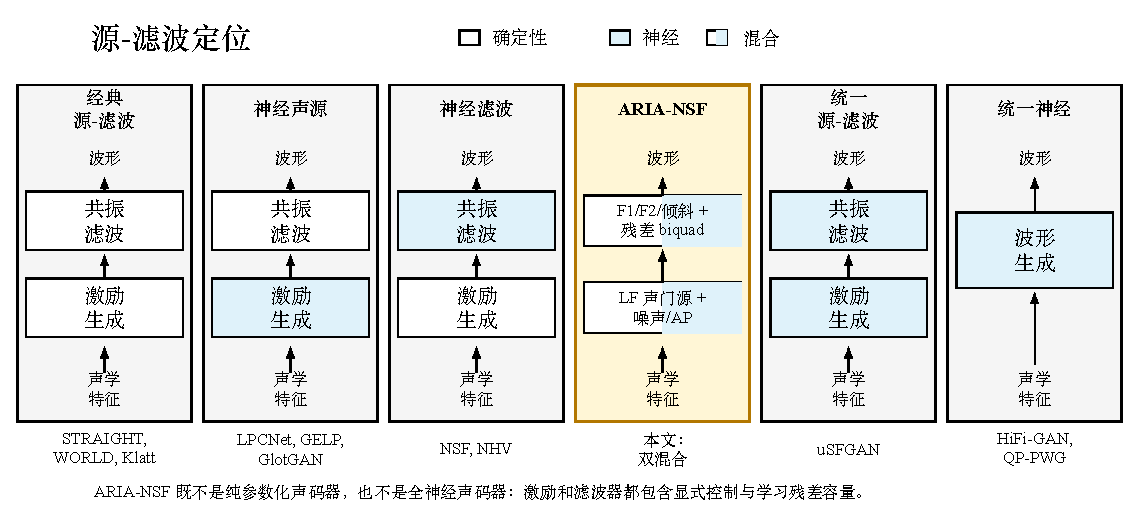
\includegraphics[width=1\linewidth,height=\textheight,keepaspectratio,alt={ARIA-NSF 在源-滤波声码器架构中的定位。该图改写自 uSFGAN 的源-滤波分类法 (Yoneyama et al. 2021)，并加入 ARIA-NSF 一列，以强调激励生成和共振滤波两者都是混合结构，而非纯确定性或纯神经结构。}]{figures/aria_source_filter_positioning_tikz_zh.pdf}
\caption{ARIA-NSF 在源-滤波声码器架构中的定位。该图改写自 uSFGAN
的源-滤波分类法 (\citeproc{ref-yoneyama2021usfgan}{Yoneyama et al.
2021})，并加入 ARIA-NSF
一列，以强调激励生成和共振滤波两者都是混合结构，而非纯确定性或纯神经结构。}
\end{figure}

这个定位也解释了 ARIA-NSF 与 GOLF、HiFi-Glot 和 uSFGAN 的差异。它不像
GOLF 那样主要服务歌声合成，也不像 uSFGAN 或 HiFi-GAN
风格系统那样把波形生成统一交给大容量神经模块；它把可编辑的语音学变量留在显式
DSP 层，同时只把残差声源和残差频谱细节分配给较小的学习模块。

\section{3.
问题设定与设计需求}\label{ux95eeux9898ux8bbeux5b9aux4e0eux8bbeux8ba1ux9700ux6c42}

ARIA-NSF
围绕五个需求设计。这些需求在语音学刺激生成中常见，但在通用神经声码器中并不总是核心目标。它们分别对应后文的显式声门源、确定性共振峰段、学习残差
biquad、低耦合诊断和小规模训练设置。

\textbf{R1. 小数据可训练性。} 系统目标用例包括 5--60
分钟的单说话人录音，因为语音学语料往往是为狭窄实验问题采集的，而不是为大规模语音生成采集的。本文当前实证主要覆盖约
1 h 单说话人设置；更短数据条件仍需系统评估。

\textbf{R2. 显式干预变量。} \(F_0\)、\(F_1/F_2\)、带宽、增益、谱倾斜和
\(R_d\)
等实验变量应保持直接可编辑。它们不应只能作为生成波形的事后测量结果被恢复出来。

\textbf{R3. 低跨参数耦合。}
操控一个维度时，应尽量少扰动其他维度。例如，操控 \(F_1\) 不应显著改变
\(F_0\)、能量或声源形状线索。

\textbf{R4. 残差表达能力。}
纯解析共振峰合成可能无法捕捉自然听感所需的说话人特异频谱细节。因此架构需要有限的学习容量，但这种容量必须受到约束，以免抹除可解释性。

\textbf{R5. 实验室可获得性。} 训练应能在消费级或普通机构 GPU
上完成。这个需求是实践性的而非理论性的，但对没有长期大型 GPU
集群访问权限的语音科学实验室非常重要。

这些需求导向一种双混合源-滤波设计：确定性成分实现实验变量，而学习残差成分则建模激励和滤波器中难以解析指定的部分。

\section{4. 模型}\label{ux6a21ux578b}

图 2 给出了当前 ARIA-NSF
流程的示意图。该架构在帧级控制和采样级合成两个时间尺度上运行。帧率声学控制可以由模型预测、从数据中提取或由用户指定；这些控制随后被上采样到音频采样率，用于可微波形合成。

\begin{figure}
\centering
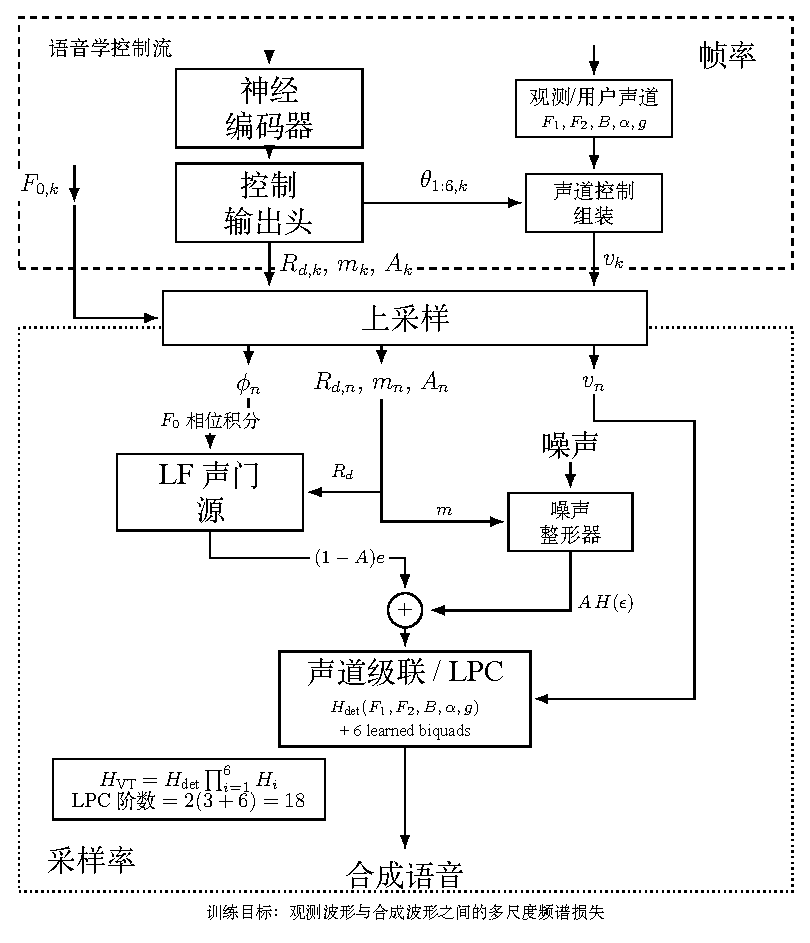
\includegraphics[width=0.8\linewidth,height=\textheight,keepaspectratio,alt={当前 ARIA-NSF 源-滤波图。所有版本先形成单一源信号再经过声道级联 / LPC；F024 v4/v6 的源信号包含带状非周期性混合 u=(1-A)e+A\textbackslash eta。}]{figures/aria_golf_f024_formula_flow_tikz_zh.pdf}
\caption{当前 ARIA-NSF 源-滤波图。所有版本先形成单一源信号再经过声道级联
/ LPC；F024 v4/v6 的源信号包含带状非周期性混合 \(u=(1-A)e+A\eta\)。}
\end{figure}

当前实验使用的编码器为 \texttt{VocoderParameterEncoderInterface}，主干为
U-Net 风格编码器加 LSTM：通道数为 \texttt{{[}32,64,128,256{]}}，四层
stride 均为 4，LSTM hidden size 为 256，层数为 3，dropout 为 0.1。F024
16 kHz 配置使用 \texttt{n\_fft=512}、hop=160，即 10 ms 帧移；\(F_0\)
范围设为 100--500 Hz。当前系统不学习 \(F_0\) 或
voicing，而是使用分析得到的真值 \(F_0\)
和清浊信息。这一点对语音学操控很重要：音高操控首先由外部指定或分析得到的
\(F_0\) 轨迹决定，而不是由高维隐变量间接恢复。

\subsection{4.1 采样率激励}\label{ux91c7ux6837ux7387ux6fc0ux52b1}

给定采样率 \(f_s\)，确定性相位轨迹通过积分帧率或采样率 \(F_0\)
轮廓得到：

\[
\phi_n = \phi_{n-1} + 2\pi \frac{F_{0,n}}{f_s}.
\]

浊音激励由 LF 风格声门源生成：

\[
e_n = g_{\mathrm{LF}}(\phi_n; R_{d,n}),
\]

其中 \(R_d\) 控制声门脉冲形状，旨在支持对 pressed 或 breathy voice
等发声类型相关维度的连续操控。该形式遵循 LF 系列声源建模的思想
(\citeproc{ref-fant1985lf}{Fant et al.
1985})，但在这里被用作神经源-滤波合成器内部的可微组件，而不是完整的独立声源模型。

噪声分支用于建模湍流或非周期能量。白噪声 \(\epsilon_n\)
经过学习或条件化的噪声整形器变换：

\[
\eta_n = H_{\mathrm{noise}}(\epsilon_n; m_n),
\]

其中 \(m_n\) 表示采样率噪声控制流。不同版本的差异主要在于谐波激励
\(e_n\) 与整形噪声 \(\eta_n\) 如何形成单一源信号。v1--v3
使用简单加性源：

\[
u_n = e_n + \eta_n.
\]

F024 主系统 v4 以及 v6 使用
\texttt{SourceFilterSynthAP}，在加性结构上加入带状非周期性（band
aperiodicity, AP）预测头：

\[
u_n = (1-A_n)e_n + A_n\eta_n,
\quad A_n(f)\in[0,1].
\]

这里 \(A_n(f)\) 表示逐频带的非周期比例。直观上，\(A\) 越接近
0，该频带越偏周期性声门源；\(A\) 越接近 1，该频带越偏整形噪声。v5 则使用
bounded noise-filter
crossfade，将同一个有界噪声滤波器同时作为噪声谱形和谐波/噪声混合权重。无论采用哪种源结构，ARIA-NSF
都先形成单一源信号 \(u_n\)，再经过一次声道 LPC 滤波；它不是分别计算
LPC(harmonic) 与 LPC(noise) 后再相加。

实现上，谐波源使用不可训练的下采样索引声门流表，\(R_d\in[0.3,2.7]\)，表长为
2048 点，使用 4 倍过采样，表类型为 LF 声门流导数，并采用 constant-power
归一化。噪声源为标准正态白噪声，随后经过时变零相位 FIR 噪声整形器；F024
16 kHz 配置中噪声幅度控制维度为 \texttt{n\_mag=128}。v4 配置额外引入 AP
预测头，旨在部分解耦噪声谱形与非周期比例；当前高频非周期性改善主要只在
v6 加入 D4C 监督后观察到，且相关数值仍需重新运行确认。

\subsection{4.2 声道级联}\label{ux58f0ux9053ux7ea7ux8054}

输出波形通过将合并后的激励送入时变声道级联滤波器得到：

\[
y_n = H_{\mathrm{VT}}(z; v_n) u_n.
\]

该滤波器被分解为确定性、可解释的段和学习残差段：

\[
H_{\mathrm{VT}}(z; v_n)
=
H_{\mathrm{det}}(z; F_{1,n}, F_{2,n}, B_{1,n}, B_{2,n}, \alpha_n, g_n)
\cdot
\prod_{i=1}^{L} H_i(z; \theta_{i,n}).
\]

每个 biquad 段可写作全极点共振器：

\[
H_i(z; \theta_i)
=
\frac{G_i}{1+a_{i,1}z^{-1}+a_{i,2}z^{-2}}.
\]

解析共振峰段使用闭式极点放置。给定中心频率 \(F\)、带宽 \(B\) 和采样率
\(f_s\)，共轭极点半径与角度为

\[
r=\exp(-\pi B/f_s),
\quad
\theta=2\pi F/f_s,
\]

对应的全极点 biquad 分母为

\[
1-2r\cos(\theta)z^{-1}+r^2z^{-2}.
\]

谱倾斜被实现为一阶实极点退化 biquad，分母为
\(1-\alpha z^{-1}\)。所有解析段和学习 biquad
并不在时域逐段串联反传，而是在系数域合成为单个 AR 多项式
\(A_{\mathrm{LPC}}(z)\)，再用一次 sample-wise LPC 施加
\(1/A_{\mathrm{LPC}}(z)\)。这样保留了级联滤波器的解释方式，同时降低高 Q
段串联带来的数值风险。

在 F024 16 kHz 主配置 v4 中，确定性成分包含三个 biquad
段，学习残差成分包含 \(L=6\) 个 biquad。对应的 LPC 等效阶数为：

\[
\mathrm{order}_{16k} = 2(3+6)=18.
\]

这里的 18 是实现中的名义 LPC 阶数；由于谱倾斜段是一阶实极点退化
biquad，有效非零极点数少一个。22/24 kHz 的 v1/v3/v4/v5
配置为了覆盖更宽频带使用 \(L=8\)，对应名义
\(\mathrm{order}=2(3+8)=22\)；v2 因关闭谱倾斜使用九个学习
biquad，同样保持名义 22 阶。因此，本文的``混合''不是一个固定的 50/50
参数比例，而是在不同采样率和数据条件下将低阶可解释声道结构与有限残差容量组合起来。该配置旨在使首要的共振峰相关自由度保持显式可控，同时保留足够的残差容量，用于学习难以手工编码的说话人特异频谱细节。

\subsection{4.3 训练目标}\label{ux8badux7ec3ux76eeux6807}

先导实现被训练为复制合成模型，使用多尺度频谱重建目标：

\[
\mathcal{L}_{\mathrm{MSSTFT}}
=
\sum_{r\in\mathcal{R}}
\left(
\left\| |S_r(x)|-|S_r(y)| \right\|_1
+
\left\| \log(|S_r(x)|+\epsilon)-\log(|S_r(y)|+\epsilon) \right\|_1
\right),
\]

其中 \(x\) 是目标波形，\(y\) 是合成波形，\(S_r\) 是分辨率为 \(r\) 的
STFT 算子。该目标与 DDSP 和神经源-滤波模型中常用的频谱损失设计一致
(\citeproc{ref-engel2020ddsp}{Engel et al. 2020};
\citeproc{ref-wang2020nsf}{Wang et al. 2020};
\citeproc{ref-yu2024golf}{Yu and Fazekas 2024})，同时保持训练过程轻量。

F024 v3/v4/v5/v6/v7 系列使用 Adam，学习率 \(2\times10^{-4}\)，gradient
clipping 为 0.5，batch size 为 128，训练 40k step。多尺度谱损失使用
\texttt{{[}127,255,511,1023{]}} 四个 FFT 尺度。共振峰监督权重为
2.0，平滑项权重为 0.05，残差正则权重为 0.02。其中 v6 复用 v4
decoder，并额外加入 D4C band-aperiodicity 监督，权重为 2.0。v1
使用较早的 200k step / batch 64 设置；v2 使用 80k step / batch
64，且关闭谱倾斜并收窄共振峰范围。这个谱系使后续比较必须区分架构变化、训练步数和监督项变化，而不能把
v2 到 v4 简化为``更多数据''或``更大模型''。

\section{5.
数据、版本与训练条件}\label{ux6570ux636eux7248ux672cux4e0eux8badux7ec3ux6761ux4ef6}

当前实验以 F024 单说话人普通话材料为主。F024 系列使用 16 kHz 采样率、10
ms 帧移，并按约 1 h
单说话人训练材料组织。为了检查架构在不同采样率和语料类型上的稳定性，实验记录还包含
CSMSC 24 kHz 和 LJSpeech 22.05 kHz 两个单说话人数据集；其中 CSMSC/LJ 的
v2/v3 使用 1 h 设置，v4/v5 使用 5 h
设置。因此，跨数据集比较主要用于判断趋势和失败模式，不能直接解释为同一数据量下的公平模型排名。

F024 版本谱系见表 1。v1--v3 主要改变解析声道约束和共振峰监督；v4/v5
改变激励中的周期/非周期处理；v7/v7b 则探索从全极点声道扩展到带零点的
ARMA 声道，以支持反共振和鼻化操控。本文以 v4 作为当前主要 F024
系统，因为它在保持 v3 声道结构的同时加入了显式 AP 预测头。

表 1. F024 16 kHz 版本谱系。

{\def\LTcaptype{none} % do not increment counter
\begin{longtable}[]{@{}
  >{\raggedright\arraybackslash}p{(\linewidth - 8\tabcolsep) * \real{0.2000}}
  >{\raggedright\arraybackslash}p{(\linewidth - 8\tabcolsep) * \real{0.2000}}
  >{\raggedright\arraybackslash}p{(\linewidth - 8\tabcolsep) * \real{0.2000}}
  >{\raggedright\arraybackslash}p{(\linewidth - 8\tabcolsep) * \real{0.2000}}
  >{\raggedright\arraybackslash}p{(\linewidth - 8\tabcolsep) * \real{0.2000}}@{}}
\toprule\noalign{}
\begin{minipage}[b]{\linewidth}\raggedright
版本
\end{minipage} & \begin{minipage}[b]{\linewidth}\raggedright
decoder
\end{minipage} & \begin{minipage}[b]{\linewidth}\raggedright
声道结构
\end{minipage} & \begin{minipage}[b]{\linewidth}\raggedright
激励/非周期处理
\end{minipage} & \begin{minipage}[b]{\linewidth}\raggedright
训练设置
\end{minipage} \\
\midrule\noalign{}
\endhead
\bottomrule\noalign{}
\endlastfoot
v1 & SF & tilt + F1/F2 + 6 learned & harmonic + noise & 200k, b64 \\
v2 & SF & 无 tilt，F1/F2 收窄，7 learned & harmonic + noise & 80k,
b64 \\
v3 & SF & 恢复 tilt，F1/F2 回到 v1，6 learned & harmonic + noise & 40k,
b128 \\
v4 & SF-AP & 同 v3 & harm + H(noise) + AP \(A(f)\) & 40k, b128 \\
v5 & SF & 同 v3 & bounded noise-filter crossfade & 40k, b128 \\
v6 & SF-AP & 同 v4 & v4 + D4C AP 监督 & 40k, b128 \\
v7/v7b & ARMA & v3 全极点 + learned zeros & 反共振/鼻化探索 & 40k,
b128 \\
\end{longtable}
}

表中 SF 表示 \texttt{SourceFilterSynth}，SF-AP 表示
\texttt{SourceFilterSynthAP}，ARMA 表示
\texttt{VocalTractCascadeARMA}；b64/b128 表示 batch size；tilt
指谱倾斜段；learned 指学习 biquad 段；AP 指带状非周期性。

模型规模保持在实验室可承受范围内。F024 v1 日志记录约 5.5M 可训练参数，v4
约 5.6M 可训练参数（约 22.2 MB），v7 约 5.5M。CSMSC/LJ 的 22/24 kHz v4
配置约 6.2M 可训练参数。声门表作为 buffer
存在，不计入可训练参数。这个规模使模型适合单说话人、小数据复制合成实验，也适合快速迭代消融。

\section{6. 先导评估结果}\label{ux5148ux5bfcux8bc4ux4f30ux7ed3ux679c}

评估同时关注合成质量和操控有效性。对语音学刺激生成而言，这两个维度同样重要。一个听起来自然但无法控制目标变量的系统并不适合受控实验；同样，一个控制精确但听感不自然的刺激也可能无法支持生态有效的听辨行为。

训练和评测围绕三类操作组织。第一类是复制合成，即从分析或预测的控制流重建训练/评测话语；第二类是参数操控，即修改
\(F_0\)、\(F_1/F_2\)、\(R_d\)
或能量后检查目标跟踪误差；第三类是耦合诊断，即在扰动一个控制维度时测量其他声学维度是否随之变化。除非另有说明，本节所有数值均为内部重建或训练快照评测，尚非
held-out
泛化结果；样本量较小，未报告统计显著性。当前结果应被理解为先导证据和失败模式记录，而不是最终基准测试或人类听感结论。

\subsection{6.1
操控保真度与参数耦合}\label{ux64cdux63a7ux4fddux771fux5ea6ux4e0eux53c2ux6570ux8026ux5408}

对操控任务，核心指标是目标跟踪误差。对共振峰而言：

\[
E_{F_i}
=
\frac{1}{T}
\sum_t
\left|
\widehat{F_i}(y_t)-F_i^{\mathrm{target}}(t)
\right|,
\quad i\in\{1,2\}.
\]

同样的逻辑也可应用于
\(F_0\)、强度、谱倾斜，以及任何估计得到的嗓音质量相关量。为了测量不期望的耦合，可以计算操控交叉效应矩阵。例如，在操控
\(F_1\) 时，分析不仅应报告 \(F_1\) 误差，还应报告由此引起的
\(F_0\)、\(F_2\)、能量、谱倾斜和 \(R_d\) 相关测量变化。

表 2 汇总了 F024 上的 measured-vs-target 斜率和 \(R^2\)。这些结果来自
\texttt{aria\_v2\_manip}
评测，N=10，随机性较大；因此表中的差异应作为趋势而不是最终排序。结果显示，\(F_2\)
操控在所有版本上都接近线性目标跟踪（\(R^2\approx0.98\)--0.99，斜率接近
1）。\(F_1\) 在 F024 上仍有系统性欠冲，v1/v2 欠冲更明显，v3 之后改善到
\(R^2\approx0.89\)--0.91、斜率约 0.88--0.90。当前证据支持 F1/F2
控制通道可用，但不支持精确独立操控的最终结论；v4
没有显著牺牲共振峰目标跟踪趋势。

表 2. F024 共振峰操控保真度与标量泄漏。

{\def\LTcaptype{none} % do not increment counter
\begin{longtable}[]{@{}lrrr@{}}
\toprule\noalign{}
模型 & F1 \(R^2\) / slope & F2 \(R^2\) / slope & 标量泄漏 \\
\midrule\noalign{}
\endhead
\bottomrule\noalign{}
\endlastfoot
v1 & 0.777 / 0.56 & 0.926 / 0.94 & 0.123 \\
v2 & 0.807 / 0.65 & 0.982 / 0.99 & 0.093 \\
v3 & 0.913 / 0.90 & 0.985 / 1.01 & 0.101 \\
v3+GAN & 0.900 / 0.90 & 0.984 / 1.00 & 0.107 \\
v4 & 0.890 / 0.88 & 0.986 / 1.00 & 0.093 \\
v5 & 0.902 / 0.88 & 0.988 / 0.97 & 0.082 \\
\end{longtable}
}

表中标量泄漏为操控交叉效应的聚合诊断量，越低表示非目标维度扰动越小；由于
N=10 且自动测量存在误差，该列只用于趋势判断。

更细的 5×5 独立性矩阵目前只对 v1、监督极点消融和 CSMSC v1
有完整记录，不能直接宣称为 v4 结果。除 F024 v1 unsup 中 F2→F1
的共振峰跟踪器异常外，已有矩阵显示 \(F_0\)、\(F_1\)、\(F_2\)
多数交叉项较低；但以 \(R_d\) 相关 alpha-ratio 度量的 tilt
与能量存在较强耦合。v4 尚需重新运行同一矩阵。因此，本文把
\(F_0/F_1/F_2\) 的低耦合作为较强但仍待统一验证的主张，把
\(R_d\)/能量的独立操控作为仍待改进的问题。

\subsection{6.2
复制合成质量}\label{ux590dux5236ux5408ux6210ux8d28ux91cf}

复制合成质量使用 MCD、LSD、MSS-STFT loss 和 SNR 等客观指标。表 3 给出
F024 的主要结果。这些是 N=50 重建/训练快照样本的描述性指标，未报告
held-out 置信区间或统计检验。在当前描述性评测中，v4 的 MCD、LSD 和
MSS-STFT 数值最低；v6 的高频周期性有所改善，但整体 MCD 不如
v4。需要注意的是，MCD 版本间差异约 0.2
dB，接近或低于常用可感知差异量级，因此不应过度解释细小排序。SNR
在当前分析-复制合成设置下均为负值，主要反映相位和激励失配，因此不宜作为主要优势或核心证据。

表 3. F024 复制合成客观指标（N=50 描述性重建评测）。

{\def\LTcaptype{none} % do not increment counter
\begin{longtable}[]{@{}lrrrr@{}}
\toprule\noalign{}
模型 & MCD↓ & LSD↓ & MSS-STFT↓ & SNR（诊断） \\
\midrule\noalign{}
\endhead
\bottomrule\noalign{}
\endlastfoot
v1 & 3.87 & 7.32 & 3.52 & -2.74 \\
v3 & 3.91 & 7.39 & 3.50 & -2.56 \\
v4 & \textbf{3.72} & \textbf{7.29} & \textbf{3.38} & -2.63 \\
v5 & 3.95 & 7.44 & 3.45 & -2.50 \\
v6 & 3.81 & 7.35 & 3.46 & -2.55 \\
\end{longtable}
}

MSS-STFT 表示多尺度 STFT 重建损失。跨语料的 MCD 结果同样显示 v4
在当前实验组合中数值较低：CSMSC 上 v4 为 3.52，低于 v1 3.66、v3 3.80 和
v5 3.83；LJSpeech 上 v4 为 3.98，低于 v1 4.08、v3 4.27 和 v5 4.33。不过
CSMSC/LJ 的 v4/v5 使用 5 h 训练材料，而 v1/v3 使用 1
h，故这些数值只能支持``v4
配置在当前实验组合中表现较好''，不能单独证明架构优越性。

\subsection{6.3
代理自然度指标}\label{ux4ee3ux7406ux81eaux7136ux5ea6ux6307ux6807}

表 4 汇总 UTMOS 代理自然度结果，每个系统 \(n=50\)。UTMOS
是神经代理模型，不等价于人类 MOS；F024 为 16 kHz，而 UTMOS
更偏向宽带语音，因此绝对值不宜跨语料解释。UTMOS
仅作为代理自然度诊断；跨语料和跨训练时长的数值不可用于架构归因。更稳妥的读法是在同一语料内比较合成系统与自然语音参考的差距。

表 4. UTMOS 代理自然度（均值±标准差，n=50）。

{\def\LTcaptype{none} % do not increment counter
\begin{longtable}[]{@{}
  >{\raggedright\arraybackslash}p{(\linewidth - 10\tabcolsep) * \real{0.1304}}
  >{\raggedleft\arraybackslash}p{(\linewidth - 10\tabcolsep) * \real{0.1739}}
  >{\raggedleft\arraybackslash}p{(\linewidth - 10\tabcolsep) * \real{0.1739}}
  >{\raggedleft\arraybackslash}p{(\linewidth - 10\tabcolsep) * \real{0.1739}}
  >{\raggedleft\arraybackslash}p{(\linewidth - 10\tabcolsep) * \real{0.1739}}
  >{\raggedleft\arraybackslash}p{(\linewidth - 10\tabcolsep) * \real{0.1739}}@{}}
\toprule\noalign{}
\begin{minipage}[b]{\linewidth}\raggedright
数据集
\end{minipage} & \begin{minipage}[b]{\linewidth}\raggedleft
自然语音
\end{minipage} & \begin{minipage}[b]{\linewidth}\raggedleft
v1/GOLF
\end{minipage} & \begin{minipage}[b]{\linewidth}\raggedleft
v2
\end{minipage} & \begin{minipage}[b]{\linewidth}\raggedleft
v4
\end{minipage} & \begin{minipage}[b]{\linewidth}\raggedleft
v5
\end{minipage} \\
\midrule\noalign{}
\endhead
\bottomrule\noalign{}
\endlastfoot
F024 16k & 2.696±0.678 & 2.422±0.632 & 2.400±0.593 & 2.526±0.634 &
\textbf{2.527±0.635} \\
CSMSC 24k & 3.901±0.370 & 3.160±0.423 & 2.986±0.393 &
\textbf{3.351±0.442} & 2.823±0.334 \\
LJ 22k & 4.370±0.088 & 3.653±0.284 & 3.427±0.313 & \textbf{4.002±0.228}
& 3.530±0.275 \\
\end{longtable}
}

粗体为同一数据集内最佳合成系统；自然语音列不参与模型排序。结果显示，v4
在 CSMSC 和 LJSpeech 当前训练配方中数值较高；F024 上 v4 与 v5
实质持平，并高于 v1/v2。DNSMOS 和 SQUIM
等非侵入式指标在当前输出上区分度较低，不作为主要证据。最终结论仍需要人类听测验证。

\subsection{6.4
高频非周期性与鼻化探索}\label{ux9ad8ux9891ux975eux5468ux671fux6027ux4e0eux9f3bux5316ux63a2ux7d22}

F024 上存在一个高频过周期问题：3--7 kHz 和 5--7 kHz
频带中，合成音频相对参考语音表现出过量谐波结构。v6 通过 D4C
非周期性监督将 3--7 kHz 过量从约 +0.044 降至
+0.028，但这些数值目前主要来自文档记录，缺少完整 slurm
日志佐证，正式论文中应重新运行实验并保存完整日志与结果。高频周期性结果目前应视为失败模式记录，不作为
v4/v6 的正式性能结论。跨语料观察还显示方向并不一致：F024
往往高频过量，而 CSMSC/LJ
可能高频不足。因此，高频非周期性不能用一个统一补偿策略解决。

v7/v7b 的 ARMA 声道用于探索鼻化和反共振。聚合指标上，鼻音和非鼻音句子的
MCD 差异很小（约 +0.01--0.04 dB），UTMOS
甚至对鼻音句给出更高分数，因此``全极点模型难以充分建模鼻音''并不会自然体现在常规重建指标中。v7b
在探针和 demo
连续体中显示可产生反共振缺口，例如低频零点比例和窄带零点比例上升，并在
demo 鼻化连续体中使 F1 区峰下降约 18 dB，而 F2
以上较少变化。这只是可控性线索，尚未构成鼻化感知或鼻化声学充分评估。

\subsection{6.5
后续感知评估}\label{ux540eux7eedux611fux77e5ux8bc4ux4f30}

正式感知评估仍然需要完成。对复制合成，可以使用 MUSHRA-like 或 CMOS
听感测试，将 ARIA-NSF 与自然录音、Praat/LPC 复制合成，以及 DDSP
harmonic-plus-noise 或 HiFi-Glot
风格源-滤波系统进行比较。对操控任务，评估应以任务为中心，而不仅仅是自然度评估。合适的设计包括：沿
\(F_1/F_2\) 元音连续统进行辨认或好坏评分测试；沿 \(F_0\)
连续统进行声调或语调感知测试；沿 \(R_d\)
连续统进行嗓音质量评分测试；使用 ABX 或 oddity
测试评估听者感知到的是目标维度而非伪影。关键标准是：合成刺激是否支持实验所要检验的同一语音学对立。

\section{7. 讨论与限制}\label{ux8ba8ux8bbaux4e0eux9650ux5236}

ARIA-NSF
的动机来自两个成熟传统之间的空缺。经典共振峰合成为语音学家提供透明控制，但听起来可能不自然。神经声码器提供高质量音频，但其控制变量往往对实验刺激生成而言过于纠缠。可微
Klatt
风格神经源-滤波模型提供了一条中间路径：保持实验上有意义的变量显式可控，同时学习自然度所需的残差结构。

对语音科学家而言，主要优势是实验控制。\(F_0\)、\(F_1/F_2\)、谱倾斜、强度和
\(R_d\)
可以作为干预变量处理，而不是作为生成波形的事后测量值。不过现有证据对这些变量的支持程度并不相同：\(F_2\)
目标跟踪较强，\(F_1\) 仍有欠冲，\(R_d\) 相关 alpha-ratio
与能量之间还存在明显耦合。对机器学习研究者而言，该模型是结构化归纳偏置的一个例子：通过将源-滤波假设放入架构，系统可以在大型黑箱神经声码器并不适合的数据规模下运行。

先导结果支持这个中间路径，但也显示出边界。v4 在 F024
描述性复制合成指标上数值较稳，并且不明显破坏 \(F_1/F_2\)
目标跟踪；跨语料 UTMOS 代理指标也显示 v4
在当前训练配方中数值较高。然而，这些结果还不能被写成最终自然度、泛化能力或架构优越性结论。首先，当前自然度主要来自
UTMOS、DNSMOS、SQUIM
等代理指标，而不是人类听测。其次，若干评估是在训练集句子或重建快照上完成，不能代表
held-out 泛化能力。第三，某些详细独立性矩阵来自 v1、监督极点消融或 CSMSC
v1，而不是 v4；因此文中必须明确每个数字对应的模型和数据集。

学习 biquad
级联既有用，也有潜在风险。它提升表达能力并改善说话人特异频谱建模，但也可能重新引入本应保持独立的参数之间的耦合。现有泄漏结果提示
\(F_0/F_1/F_2\) 多数交叉项较低，而 \(R_d\) 相关 alpha-ratio
与能量之间仍有明显耦合。未来工作应直接分析学习段，例如跟踪极点轨迹、检查共振峰交互，并对学习残差级联进行消融。v7/v7b
的 ARMA 扩展也提示，常规 MCD/UTMOS
指标可能看不出鼻化问题；如果目标是可控鼻化，应设计针对反共振缺口、鼻腔
murmur 和 A1-P0 线索的专门评估。

因此，当前先导实现应被理解为一个系统论文和先导评测，而不是标准化基准评测。本文最强主张是架构与可运行性：语音学刺激生成可能受益于让实验上有意义的参数保持解析，同时只把残差声源和残差频谱细节分配给学习模块。经验结果目前只支持先导性可行性和失败模式识别；最终自然度、泛化能力和架构优越性仍需通过与
Praat/LPC 操控、DDSP 风格 harmonic-plus-noise
合成，以及更强的神经源-滤波或 HiFi-Glot
风格模型进行受控比较来进一步支撑。

\section{8. 结论}\label{ux7ed3ux8bba}

本文介绍了 ARIA-NSF，一种面向小数据语音学刺激生成的可微 Klatt
风格神经源-滤波合成器。该模型将确定性声源建模、显式共振峰控制和学习残差频谱建模结合起来，旨在保留经典共振峰合成的可解释性，同时提升复制合成质量和参数操控后刺激材料的可用性。当前
F024 主配置 v4 使用 LF 风格声门激励、整形噪声、AP
混合权重，以及由确定性全极点段和六个学习 biquad 组成的声道级联，名义 LPC
阶数为 18。先导评测显示，v4 在 F024 描述性复制合成评测中 MCD/MSS-STFT
数值较低，并在 F1/F2
操控中保持较高目标跟踪趋势。下一步是完成严格的人类听测、重新运行并统一关键评估口径，并将训练集重建结果扩展到清晰的
held-out 泛化评估。

\section{致谢}\label{ux81f4ux8c22}

先导录音是在北京语言大学张劲松老师课题组相关工作期间采集的。作者感谢早期神经源-滤波、DDSP、GOLF
和神经共振峰合成工作对这一混合设计的启发。

\section{数据可用性}\label{ux6570ux636eux53efux7528ux6027}

当前先导语料包含为语音学研究采集的语音录音，尚未公开发布。包含若干复制合成和操控示例的演示页面可见于
\url{https://n1r.github.io/ARIA_nsf/}。

\section{伦理声明}\label{ux4f26ux7406ux58f0ux660e}

未来的感知评估将需要听者知情同意，并需要适当处理说话人录音。本文草稿不报告任何感知听者数据。

\section{作者贡献}\label{ux4f5cux8005ux8d21ux732e}

Yiran Ding 设计模型、准备先导语料、实现当前系统并撰写本文草稿。

\section{利益冲突}\label{ux5229ux76caux51b2ux7a81}

作者声明不存在利益冲突。

\section{资助}\label{ux8d44ux52a9}

当前先导工作未报告专门资助。

\section{AI 辅助声明}\label{ai-ux8f85ux52a9ux58f0ux660e}

本文使用了 AI
写作辅助来组织草稿结构并润色语言。作者对所有技术主张、实验和最终稿件内容负责。

\section*{参考文献}\label{ux53c2ux8003ux6587ux732e}
\addcontentsline{toc}{section}{参考文献}

\protect\phantomsection\label{refs}
\begin{CSLReferences}{1}{1}
\bibitem[\citeproctext]{ref-boersma2001praat}
Boersma, Paul. 2001. {``Praat, a System for Doing Phonetics by
Computer.''} \emph{Glot International} 5 (9/10): 341--45.

\bibitem[\citeproctext]{ref-engel2020ddsp}
Engel, Jesse, Lamtharn Hantrakul, Chenjie Gu, and Adam Roberts. 2020.
{``DDSP: Differentiable Digital Signal Processing.''}
\emph{International Conference on Learning Representations}.
\url{https://openreview.net/forum?id=B1x1ma4tDr}.

\bibitem[\citeproctext]{ref-fant1960acoustic}
Fant, Gunnar. 1960. \emph{Acoustic Theory of Speech Production}. (The
Hague).

\bibitem[\citeproctext]{ref-fant1985lf}
Fant, Gunnar, Johan Liljencrants, and Qi-Guang Lin. 1985. {``A
Four-Parameter Model of Glottal Flow.''} \emph{STL-QPSR} 26 (4): 1--13.

\bibitem[\citeproctext]{ref-gu2026hifiglot}
Gu, Yicheng, Pablo Perez Zarazaga, Chaoren Wang, et al. 2026.
{``HiFi-Glot: High-Fidelity Neural Formant Synthesis with Differentiable
Resonant Filters.''} \emph{arXiv:2409.14823}.
\url{https://arxiv.org/abs/2409.14823}.

\bibitem[\citeproctext]{ref-klatt1980software}
Klatt, Dennis H. 1980. {``Software for a Cascade/Parallel Formant
Synthesizer.''} \emph{The Journal of the Acoustical Society of America}
67 (3): 971--95. \url{https://doi.org/10.1121/1.383940}.

\bibitem[\citeproctext]{ref-wang2020nsf}
Wang, Xin, Shinji Takaki, and Junichi Yamagishi. 2020. {``Neural
Source-Filter Waveform Models for Statistical Parametric Speech
Synthesis.''} \emph{IEEE/ACM Transactions on Audio, Speech, and Language
Processing} 28: 402--15.
\url{https://doi.org/10.1109/TASLP.2019.2956145}.

\bibitem[\citeproctext]{ref-yoneyama2021usfgan}
Yoneyama, Reo, Yi-Chiao Wu, and Tomoki Toda. 2021. {``Unified
Source-Filter GAN: Unified Source-Filter Network Based on Factorization
of Quasi-Periodic Parallel WaveGAN.''} \emph{arXiv:2104.04668}.
\url{https://arxiv.org/abs/2104.04668}.

\bibitem[\citeproctext]{ref-yu2024golf}
Yu, Chin-Yun, and Gyorgy Fazekas. 2024. {``GOLF: A Singing Voice
Synthesiser with Glottal Flow Wavetables and LPC Filters.''}
\emph{Transactions of the International Society for Music Information
Retrieval} 7 (1): 316--30. \url{https://doi.org/10.5334/tismir.210}.

\end{CSLReferences}
